\markdownRendererHeadingFour{Distribuciones de precios}\markdownRendererInterblockSeparator
{}Al comparar con las distribuciones de retornos generadas por la misma serie de precios se observa que al añadir mayor proporción de agentes MA las colas de las distribuciones de retornos se hacen cada vez más pesadas, lo cual es una propiedad deseable de una simulación de un mercado.\markdownRendererInterblockSeparator
{}\begin{figure}[h!] \centering 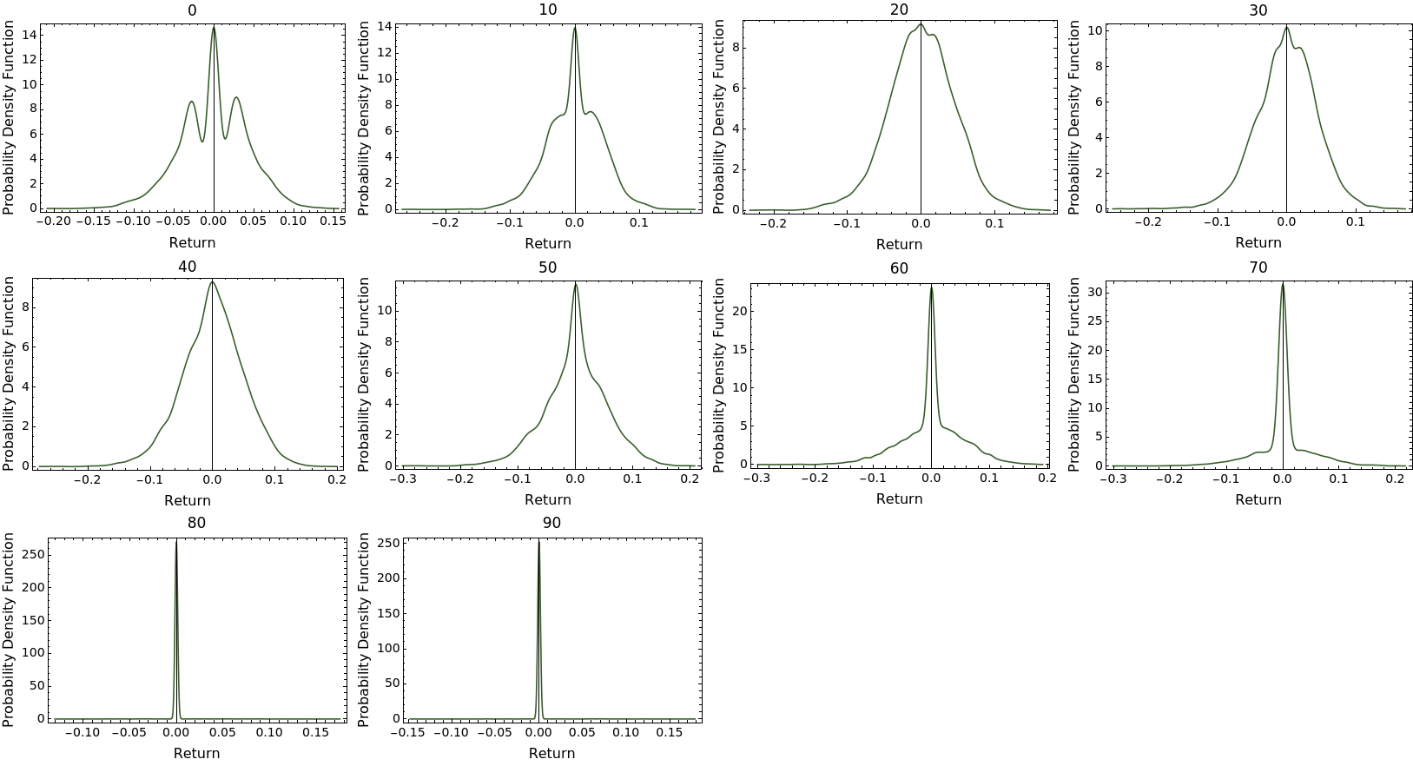
\includegraphics[scale=0.25]{img/dist_prices.png} \end{figure}\markdownRendererInterblockSeparator
{}\markdownRendererHorizontalRule{}\markdownRendererInterblockSeparator
{}\markdownRendererHeadingFour{Comparación de estrategias}\markdownRendererInterblockSeparator
{}Comparando la riqueza promedio de los agentes tipo MA con los ZI es posible concluir que la estrategia MA genera una ventaja significativa con respecto a la estrategia ZI.\markdownRendererInterblockSeparator
{}\begin{figure}[h!] \centering 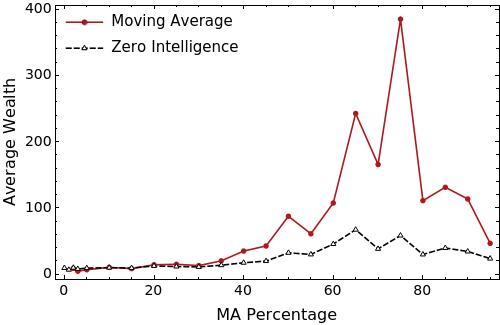
\includegraphics[scale=0.4]{img/wealth_comparison.jpeg} \end{figure}\markdownRendererInterblockSeparator
{}\markdownRendererHorizontalRule{}\relax